\subsection[]{Dimostrare che il raggio nucleare si può ricavare tramite la misura del fattore di forma elettromagnetico di un nucleo utilizzando elettroni veloci. Indicare quali angoli di scattering devono essere coperti dalla strumentazione nel caso di elettroni di energia 1 GeV su un nucleo di Piombo.}%
\label{sec:5.c.36}
Tutti i grafici riportati in questa sezione fanno riferimento ai dati del problema.\\
Partiamo dallo Scattering Mott:
\[
	\left.\frac{\mbox{d}\sigma }{\mbox{d} \Omega} \right|_{\text{Mott}} = 
		\left[ 1- \beta^2 \sin^2\left( \frac{\theta}{2} \right) \right]\cdot \left.\frac{\mbox{d} \sigma}{\mbox{d} \Omega} \right|_{\text{Rutherford}} 
.\] 
In cui vi è una correzione allo scattering Rutherford, che ricordiamo essere:
\[
	\left.\frac{\mbox{d} \sigma}{\mbox{d} \Omega} \right|_{\text{Rutherford}}= \left( \frac{zZe^2}{4\pi\epsilon_0} \right)^2\left( \frac{1}{4T} \right)^2 
		\frac{1}{\sin^4\left( \frac{\theta}{2} \right) }
.\] 
Dove $T$ è l'energia cinetica della particella incidente, esprimibile anche come $T = pV /2$.
L'andamento del Mott al variare di $\theta$ è:
\begin{figure}[H]
	\centering
	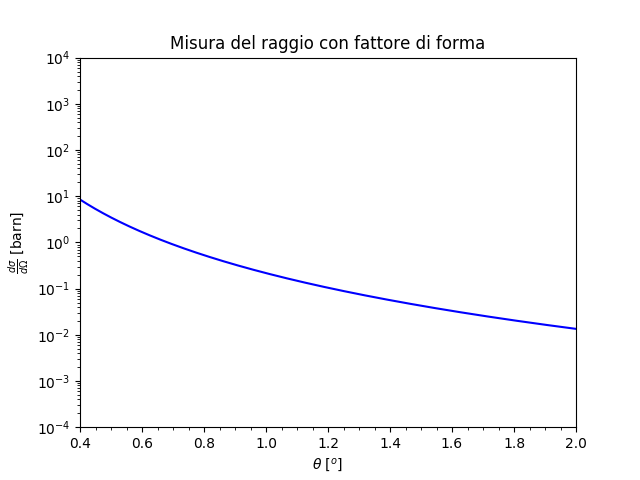
\includegraphics[width=0.6\textwidth]{immagini/Mott.png}
	\caption{Sezione d'urto Mott differenziale}
	\label{fig:immagini-Mott-png}
\end{figure}
Quello che vorremmo noi è essere in grado di dare una dimensione al centro scatterante, con le sole formule scritte sopra non potremmo farlo perchè entrambi gli scattering si riferiscono a nuclei puntiformi. Per poter correggere lo scattering Mott dobbiamo ipotizzare che il nucleo sia sferico, in tal modo il calcolo effettuato per ottenere la sezione d'urto Mott resta valido (per il teorema della media se si vuole) e quando si considera il campo generato dalla carica Q bersaglio dobbiamo considerare il campo di una carica puntiforme con la correzione: 
\[
	Q = F\left(\bs{q}\right)\int\rho\left(\bs{r}\right)d^3r = F\left(\bs{q}\right) Ze 
\]
Dove si aggiunge il fattore di forma per tener di conto della interferenza di ogni elemento infinitesimo della carica Q vista da un osservatore lontano. A questo punto la sezione d'urto sul nucleo diventa:
\[
	\frac{\mbox{d} \sigma}{\mbox{d} \Omega} =
		\left|Z F\left( \bs{q} \right)  \right|^2\left[ 1- \beta^2\sin^2\left( \frac{\theta}{2} \right)  \right]
		\cdot \left.\frac{\mbox{d} \sigma}{\mbox{d} \Omega} \right|_{\text{Rutherford}}
.\] 
Il significato fisico di $\bs{q}$ è il momento trasferito dall'elettrone (se moltiplicato per $\hbar$) durante lo scattering ed il suo modulo vale:
\[
	\left|\bs{q}\right|= 2k\sin\left(\frac{\theta}{2}\right)= 2\cdot \frac{2\pi}{\lambda}\sin\left( \frac{\theta}{2} \right) 
.\] 
Con $p$ impulso iniziale dell'elettrone. Per comprendere meglio la struttura del fattore di forma analizziamo la situazione dal punto di vista ondulatorio: la lunghezza d'onda di De Broglie dell'elettrone è $\lambda = h /p$, immaginiamo il nucleo come un ostacolo opaco di raggio R, un oggetto che faccia da barriera di potenziale per l'elettrone in modo che questo non possa penetrarvi. A titolo di esempio prendiamo il seguente modello semplificato:
\begin{figure}[H]
    \centering
    \incfig{elettrone-su-nucleo-fattore-forma}
    \caption{elettrone su nucleo}
    \label{fig:elettrone-su-nucleo-fattore-forma}
\end{figure}
Le onde che passano sopra al nucleo percorrono una distanza $2R\sin\theta$ volte maggiore rispetto a quelle che passano sotto al nucleo per arrivare al rilevatore, questo comporta che (essendo il rilevatore e la distanza dall'evento di scattering entrambi molto maggiori di tutte le distanze disegnate) quando si verifica l'uguaglianza:
\[
	2R\sin\theta = \left( n + \frac{1}{2} \right)\lambda 
.\] 
Le due onde arrivano in controfase e si ha quindi interferenza distruttiva, per tale angolo la sezione d'urto differenziale si annulla.\\
L'idea alla base è questa, in un modello più realistico dobbiamo considerare che le onde possono attraversare il nucleo, di queste onde se ne tiene di conto tramite il fattore di forma (che infatti incide direttamente sulla sezione d'urto differenziale: dove si annulla lui si annulla anche lei).\\
Il fattore di forma non è altro che la trasformata di fourier della distribuzione di carica, quindi data una carica $Q = Ze$ con distribuzione $\rho$ avente simmetria sferica si ha che il fattore di forma è del tipo: 
\[
	F\left( \bs{q} \right) = \frac{1}{Ze}\int \rho\left( \bs{r} \right) e^{i \bs{r}\cdot \bs{q}}d^3r
.\] 
Scegliendo un sistema di riferimento con cordinate sferiche l'integrale diventa:
\begin{align*}
	Q \cdot F\left( \bs{q} \right) &= 2\pi \int_{0}^{\pi} \int_{\infty}^{\infty}\rho\left( r \right) r^2e^{i rq \cos\theta}\sin\theta d\theta dr\\
	&=  2\pi \int_{-1}^{1} \int_{-\infty}^{\infty}\rho\left( r \right) r^2e^{i rq \cos\theta}\left|d\cos\theta\right|dr\\
	&=  2\pi\cdot  2 \cdot \int_{-\infty}^{\infty} \frac{e^{iqr}-e^{-iqr}}{2iqr} r^2 \rho\left( r \right) dr  \\
	&=  \frac{4\pi}{q} \int_{-\infty}^{\infty} r\sin\left( qr \right) \rho\left( r \right) dr 
.\end{align*}
Modellizziamo adesso la distribuzione di carica come:
\[
	\rho\left( \bs{r} \right) = 
	\begin{cases}
		\ 0 & \text{se } \left| \bs{r} \right| > R \\ 
		\ \frac{3Q}{4\pi R^3} & \text{se } \left| \bs{r} \right| < R 
	\end{cases}
.\] 
Ed inserita nel conto ci riporta a 
\[
	F\left( q \right) = 3\left( \frac{\sin\left( Rq \right) }{\left( Rq \right)^3}- \frac{\cos\left( Rq \right) }{\left( Rq \right)^2} \right) 
.\] 
\begin{figure}[H]
	\centering
	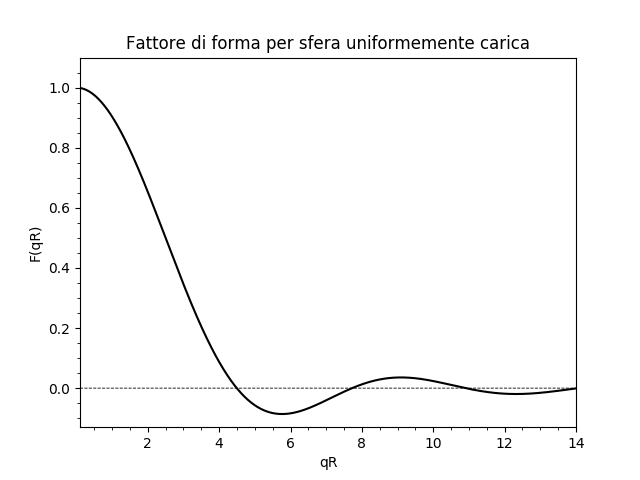
\includegraphics[width=0.5\textwidth]{immagini/Form-factor-sphere.png}
	\caption{Fattore di forma per sfera uniformemente carica}
	\label{fig:immagini-Form-factor-sphere-png}
\end{figure}
Studiando i punti in cui si annulla questo fattore di forma è possibile estrapolare informazioni sul raggio atomico, informazioni sulle quali si può fare esperimenti misurando la sezione d'urto differenziale e confrontando il primo minimo con quello atteso ottenuto numericamente (diverso dallo zero che corrisponde ad angolo nullo): 
\[
	Rq_{\text{min}} = a \approx 4.5
.\] 
Inserendo l'espressione di $q$ in funzione di angolo ed impulso:
\[
	2 \frac{p}{\hbar} \sin\left( \frac{\theta_{\text{min}}}{2} \right) R = a \implies R = \frac{a \hbar}{2 p \sin\left( \frac{\theta_{\text{min}}}{2} \right) } 
.\] 
Abbiamo quindi una espressione di $R$ in funzione dell'angolo corrispondente al primo minimo di interferenza, ipotizziamo di voler verificare che il raggio nucleare del piombo sia:
\[
	R = \left( 1.25\cdot A^{1 /3} + 2 \right)\text{ [fm]} = \left(1.25\cdot 207^{1 /3} + 2 \right)\text{ [fm]} \approx 9.4 \text{ [fm]}  
.\] 
Con elettroni come nel testo, dobbiamo trovare l'impulso di tali elettroni:
\[
	p = \sqrt{E^2-m^2} \approx 1 \text{GeV/c}	
.\] 
La costante di Plank ridotta in queste unità vale: $\hbar = 6.6 \cdot 10^{-16}$ eV$\cdot$s. Se ne conclude che per misurare il raggio nucleare del piombo dovremmo posizionare una strumentazione che sia sensibile ad angoli di scattering tali che:
\[
\frac{\theta}{2} = \arcsin \left(\frac{a \hbar}{2pR}\right) = \arcsin \left( \frac{4.5\cdot 6.6 \cdot 10^{-16}\cdot 3 \cdot 10^{8} }{2\cdot 1\cdot 10^{9}\cdot 9.4 \cdot 10^{-15}}\right) \approx 0.3^o
 .\]
 Quindi dovremmo avere una strumentazione sensibile almeno a 0.6$^o$. 
 \begin{figure}[H]
 	\centering
 	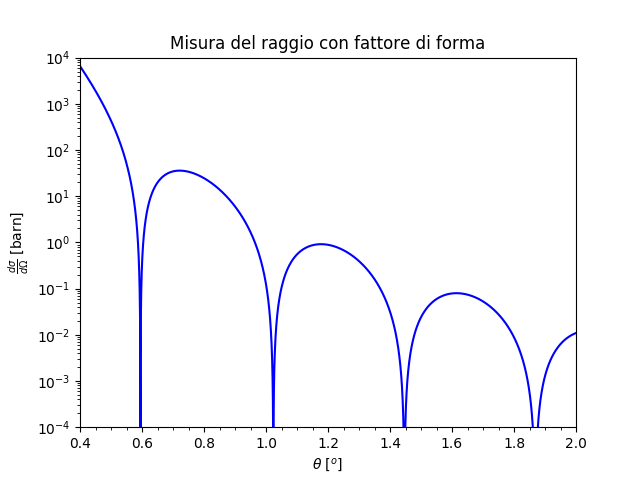
\includegraphics[width=0.6\textwidth]{immagini/misura-raggio-piombo.png}
	\caption{Sezione d'urto per un elettrone incidente su un atomo di piombo considerando $F\left( \bs{q} \right) $}
 	\label{fig:immagini-misura-raggio-piombo-png}
 \end{figure}
